\chapter{Dasar Teori}
\label{chap:definition}
Pada bab ini akan dijelsaskan mengenai konsep-konsep dasar pengukung BI, yaitu DSS(\textit{decision support system}), konsep BI(\textit{business intelligence }) itu sendiri, \textit{data warehouse} dengan OLAP(\textit{online analytical processing}), ORM(\textit{object relational mapping}), MVC(\textit{model view controller}), serta penjelaasan mengenai perangkat lunak ODOO yang digunakan untuk membangun BI \textit{tool}.

\section{Decision Support Systems}
\textit{Decision support systems} atau yang biasa disingkat DSS merupakan sebuah set pengembangan teknik IT yang interaktif atau bisa dikatakan sebagai sebuah alat yang didesain untuk menganalisis dan memproses data untuk membantu seorang manajer di suatu perusahaan dalam membuat keputusan. Dalam membuat sebuah keputusan, sistem dapat mencocokan sumber data individual dari seorang manajer dengan sumber data yang dimiliki oleh komputer sehingga dapat meningkatkan kualitas keputusan yang akan dipilih \cite{Matteo:2009}. Fungsi DSS dapat dicerminkan sebagai konsep dari pengambilan keputusan dalam kondisi yang berbeda-beda, akan sangat berguna untuk memecahkan masalah yang tidak terstruktur maupun semi terstruktur. Dimana proses pengambilan keputusan terjadi dengan adanya dialog interaktif antara DSS dan pengguna. Adanya \textit{user interface} menandakan \textit{user} tetap memegang kontrol penuh dalam pengambilan keputusan \cite{rassoblog}.   

\section{Business Intelligence}

\textit{Business Intelligence} pada hakikatnya merupakan solusi perangkat lunak bagi \textit{decision-makers} dalam perusahaan yang dapat membantu \textit{decision-makers} mengindentifikasi dan memahami kunci dari faktor bisnis yang dijalani oleh perusahaan tersebut. BI juga dapat membantu \textit{decision-makers} mengambil keputusan terbaik untuk situasi yang berlaku pada saat itu\cite{Matteo:2009}. Pengertian lain \textit{business intelligece} (BI) yaitu aplikasi
\textit{e-business} yang berfungsi untuk mengubah data dalam perusahaan (data operasional, transaksional, dan lainnya) ke dalam bentuk ringkasan informasi yang dibutuhkan. Tujuan utama dari sistem \textit{business intelligence} adalah untuk menyediakan informasi untuk dapat membuat keputusan yang tepat dan efektif. Beberapa fungsi BI di antaranya menyajikan laporan(\textit{query} dan \textit{reporting}), eksplorasi data(\textit{data mining}), analisis secara \textit{online}(\textit{online analytical processing} (OLAP)), pembandingan(\textit{benchmarking}), dan pencarian teks(\textit{text mining}). \cite{Carlo:2009}

\subsection{Arsitektur \text{business intelligence}}
Arsitektur sistem BI memiliki 3 komponen utama, yaitu \textit{data sources}, \textit{data Data warehouses} dan \textit{data marts}. Penjelasan lebih lanjut dan bentuk arsitektur BI dapat dilihat pada Gambar \textbf{2.1}.

\begin{figure}[h]
	\centering
	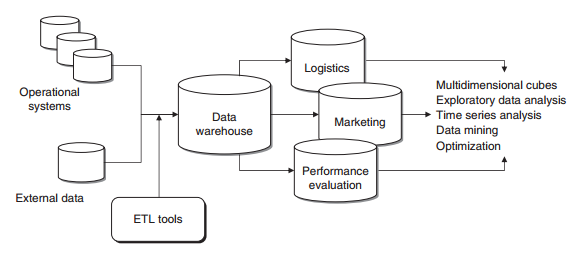
\includegraphics{Gambar/arsitekturBI}
	\caption{Komponen utama dari sistem \textit{business intelligence} \cite{Carlo:2009}}
	\end{figure}

\subsubsection{\textit{Data Sources}} Pada arsitektur BI, tahap pertama yang dilakukan adalah pengumpulan dan pengintegrasian data dari berbagai sumber dengan tipe yang beragam. Sumber data biasanya berasal dari sistem operasional. Selain itu, sumber data dapat berupa dokumen yang tidak mempunyai struktur seperti email, teks atau data eksternal lainnya.\cite{Carlo:2009}

\subsubsection{\textit{Data Warehouses} dan \textit{Data Marts}} Setelah sumber data terkumpul, selanjutnya data akan masuk dalam proses ekstrasi dan transformasi yang biasa  disebut dengan proses \textit{extract, transform, load} (ETL). Data yang telah melalui proses ETL disimpan dalam basis data sebagai  \textit{data warehouses} dan \textit{data marts}. \cite{Carlo:2009}

\subsubsection{Analisis BI}
Data yang telah melalui proses ETL dan disimpan sebagai \textit{data warehouse} kemudian di analisis oleh sistem BI. Beberapa contoh analisis BI, yaitu :
\begin{itemize}
	\item analisis \textit{multidimensional cube} merupakan analisis berbasis data array multidimensi
	\item analisis eksplorasi data merupakan analisis berupa statistik dan visual.
	\item analisis berdasarkan waktu merupakan analisis berbasis pada waktu tertentu.
	\item model pembelajaran secara induktif untuk \textit{data mining} merupakan model untuk mempelajari apa yang ada pada data.
	\item model optimisasi merupakan optomisasi untuk memilih alternatif terbaik untuk disajikan sebagai bahan pertimbangan pengambilan keputusan.
\end{itemize} 

\section{Data Warehouse}
Pada bagian ini akan dibahas mengenai pengertian dari \textit{data warehouse}, karakteristik \textit{data warehouse}, arsitektur \textit{data warehouse} serta peran \textit{data warehouse} dalam BI .

\subsection{Definisi \textit{Data Warehouse}}
Sebelum membahas lebih jauh terdapat dua tipe data yang sering dipakai oleh perusahaan yaitu data operasional dan \textit{data warehouse}. Terdapat perbedaan mendasar dari kedua data tersebut, data operasional biasanya mencakup periode waktu yang singkat, hal ini karena data operasional biasanya berisi data transaksi yang diperbarui setiap harinya. Sedangkan \textit{data warehouse} mempunyai lingkup yang lebih luas yaitu menyimpan data yang mencakup beberapa tahun untuk proses analisis. Oleh karena itu, \textit{data warehouse} diperbarui secara berkala dari data operasional agar selalu berkembang. Secara konsep \textit{Data warehouse} (DWH)   merupakan kumpulan teknik, metoda atau bisa dikatakan sebagai suatu \textit{tools} yang dapat membantu manajer, direktur maupun analis perusahaan untuk melakukan analisis data sebelum mengambil keputusan. Secara singkat \textit{data warehouse} dapat di artikan sebagai sekumpulan data yang membantu proses pengambilan keputusan. Karakteristik DWH yaitu \textit{subject-oriented}, terintegrasi, konsisten, berevolusi dari waktu ke waktu, dan tidak berubah-ubah(\textit{not volatile}) \cite{Matteo:2009}.  

\begin{figure}[h]
	\centering
	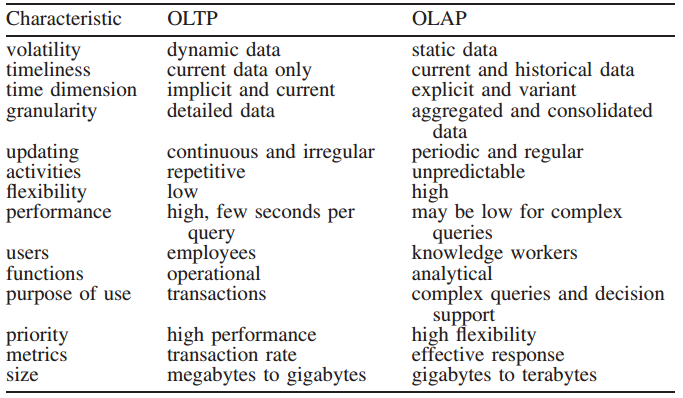
\includegraphics[scale=0.65]{Gambar/OLTP&OLAP}
	\caption{Perbedaan OLTP dan OLAP sistem \cite{Carlo:2009}}
	\end{figure}
	
	Desain \textit{data warehouse} memliliki perbedaan mendasar dengan \textit{operational databases}. Gambar \textbf{2.2} merangkum perbedaan mendasar antara OLTP(\textit{on-line transaction processing}) dan OLAP(\textit{on-line analytical processing}) sistem. 
	
\subsubsection{Karakteristik \textit{Data Warehouse}}
\textit{Data Warehouse} memiliki empat karakteristik utama, yaitu \cite{Matteo:2009}.
\begin{enumerate}
	\item \textit{Subject Oriented}\\
	\textit{Data warehouse} dirancang, dan dibangun untuk memenuhi kebutuhan analisis berdasarkan subyek tertentu. Misalnya, \textit{data warehouse} untuk \textit{customer} atau produk.
	\item \textit{Integrated}\\
	\textit{Data warehouse} mampu mengintegrasikan data sumber yang berbeda-beda kedalam format yang seragam.
	\item \textit{Non Volatile}\\
	Format data dalam sebuah \textit{data warehouse} tidak bisa diubah karena merupakan data historis, data dalam \textit{data warehouse} hanya boleh ditambah saja.
	\item \textit{Time Variant}\\
	Setiap data yang disimpan dalam \textit{data warehouse} memiliki dimensi waktu. Dimensi waktu tersebut selanjutnya akan dimanfaatkan sebagai pembanding dalam pembuatan laporan.
\end{enumerate}
	
\subsubsection{\textit{Data Marts}}

\textit{Data marts} merupakan bagian dari kumpulan data yang disimpan dalam \textit{data warehouse}.Kumpulan data tersebut mengandung satu set bagian informasi yang relevan dan merujuk ke arah area bisnis yang spesifik, seperti bagian departemen dalam suatu perusahaan atau kategori pengguna. Jadi cakupan \textit{data mart} lebih spesifik dibanding \textit{data warehouse} \cite{Matteo:2009}. Ada beberapa karakteristik dari data mart yang membedakannya dengan data warehouse, yaitu.\cite{Carlo:2009}
\begin{enumerate}
	\item Data mart lebih fokus pada kebutuhan pengguna, departemen atau fungsi bisnis.
	\item Data mart tidak  berisi data operasional yang terperinci. 
	\item Data mart berisi lebih sedikit data dari data warehouse, sehingga lebih mudah dimengerti dan dipahami.	
\end{enumerate}

\subsection{Arsitektur \textit{Data Warehouse}}
Arsitektur \textit{data warehouse} dapat dikelompokan menjadi tiga, yaitu\cite{Matteo:2009}:

\subsubsection{\textit{Single-Layer Architecture}}
\textit{Single-layer architecture} bertujuan untuk meminimalisir jumlah data yang disimpan dengan cara mengilangkan redundansi data.

\begin{figure}[h]
	\centering
	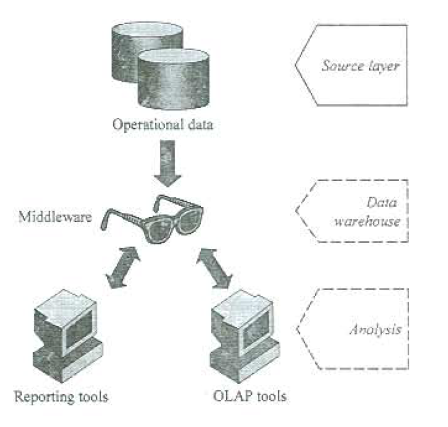
\includegraphics[scale=0.75]{Gambar/single-layer}
	\caption{Gambar \textit{Single-Layer Architecture}\cite{Matteo:2009}}
	\end{figure}
	Diterangkan pada gambar \textbf{2.3} bahwa hanya terdapat satu layer dalam arsitektur ini, yaitu \textit{source layer} yang berisi data operasional. \textit{Data warehouse} dianggap sebagai \textit{virtual layer} sehingga \textit{data warehouse} dalam konteks ini dianggap sebagai tampilan multidimensional dari data operasional yang secara spesifik disebut \textit{middleware} atau \textit{intermediate processing layer}. Kekurangan arsitektur ini terletak pada sulitnya menemukan prasyarat untuk memisahkan proses analisis dan transaksi.\cite{Matteo:2009}
	
\subsubsection{\textit{Two-Layer Architecture}}
\begin{figure}[h]
	\centering
	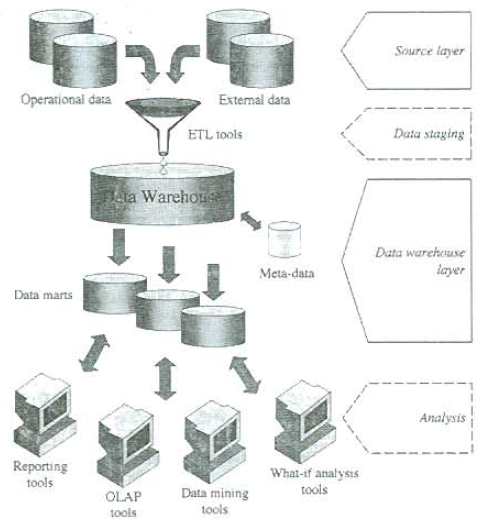
\includegraphics[scale=0.85]{Gambar/two-layer}
	\caption{Gambar \textit{Two-Layer Architecture}\cite{Matteo:2009}}
	\end{figure}
Arsitektur ini menggunakan dua layer yaitu memisahkan antara sumber data fisik dan \textit{data warehouse}. Terdapat empat bagian sebagai pendukung aliran data pada arisitektur ini, yaitu: 
\begin{enumerate}
	\item \textit{Source layer}\\
	Sebuah \textit{data warehouse} terdiri dari sumber data yang heterogen yang berasal dari data operasional perusahaan, basis data warisan, maupun data yang berasal dari luar lingkup perusahaan.
	\item \textit{Data staging}\\
	\textit{Data staging} merupakan tempat penyimpanan sementara untuk proses ETL(\textit{extract, transform, load }).
	\item \textit{Data warehouse layer}\\
	Setelah data melalui proses ETL, data akan disimpan dalam satu penyimpanan tunggal yang tersentralisasi yang disebut \textit{data warehouse}. \textit{Data warehouse} bisa digunakan sebagai sumber untuk membuat \textit{data mart} untuk kebutuhan yang lebih spesifik.
	\item Analisis\\
	Dalam layer ini, data yang terintegrasi bersifat efisien dan fleksibel untuk diakses sehingga dapat digunakan untuk membuat laporan, melakukan analisis data, dan lain-lain.
\end{enumerate}

\subsubsection{\textit{Three-Layer Architecture}}
\begin{figure}[h]
	\centering
	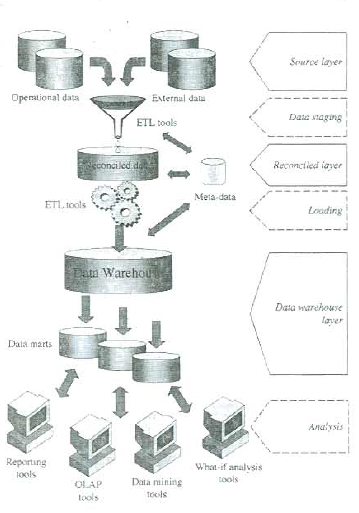
\includegraphics[scale=0.95]{Gambar/three-layer}
	\caption{Gambar \textit{Three-Layer Architecture}\cite{Matteo:2009}}
	\end{figure}
	
	Dalam arsitektur ini, terdapat layer ketiga yang disebut dengan \textit{reconciled data layer}. Layer ketiga ini tercapai ketika mendapatkan data operasional yang terintegrasi dan telah dibersihkan dari data sumbernya. Isi dari \textit{reconciled data layer} ini adalah data yang telah terintegrasi, konsisten, data yang benar, data terkini dan detil. Keuntungan dari penggunaan \textit{reconciled data layer} ini adalah terciptanya suatu model data yang dapat menjadi referensi bagi seluruh data perusahaan. Kekurangannya adalah penggunaan \textit{reconciled data layer} dapat mengarah pada redundansi pada sumber data operasional\cite{Matteo:2009}.

\subsection{Proses ETCL}
Proses mentransformasikan data sumber kedalam \textit{data warehouse} dengan berbagai macam variasi data pada sumber disebut proses ETCL. Proses ETCL terdiri dari empat tahap, yaitu \textit{extract, transform, clean,} dan \textit{load}. Proses ETCL merupakan proses utama dalam membangun \textit{data warehouse} dan \textit{data mart}. Berikut penjelasan mengenai tahapan dari ETCL dengan disertai gambar \textbf{2.6}.
\begin{figure}[h]
	\centering
	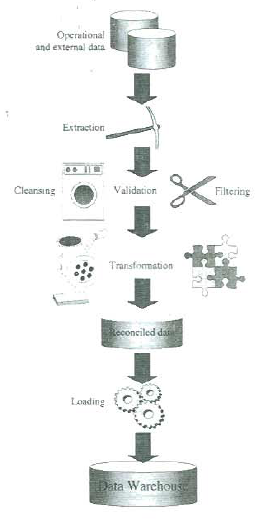
\includegraphics[scale=0.95]{Gambar/etl-proses}
	\caption{Contoh Proses ETCL Pada \textit{Data Warehouses}\cite{Matteo:2009}}
	\end{figure} 

\subsubsection{\textit{Extract}}
\textit{Data warehouse} terdiri dari berbagai sumber data. Proses ekstraksi pada ETCL berfungsi untuk mendapatkan data yang relevan sesuai dengan kebutuhan \textit{data warehouse}. Proses ekstraksi terbagi menjadi dua tipe, yaitu \cite{Matteo:2009}:

\begin{enumerate}
	\item \textit{Static extraction}\\
	\textit{Static extraction} adalah proses pengisian sebuah \textit{data warehouse} untuk pertama kali. Proses ini seperti gambaran dari data operasional.
	\item \textit{Incremental extraction}\\
	\textit{Incremental extraction} digunakan untuk proses memperbarui \textit{data warehouse} secara berkala. Poses ini juga untuk mengaplikasikan perubahan dari sumber data sejak terakhir kali proses ekstraksi.
\end{enumerate}

\subsubsection{\textit{Cleansing}}
Fase membersihkan data merupakan fase penting dalam sistem \textit{data warehouse} karena dapat meningkatkan kualitas data karena pada umumnya sumber data tidak memiliki kualitas yang memadai untuk dimasukan dalam \textit{data warehouse}. Berikut ini merupakan kesalahan yang sering dilakukan serta inkonsistensi data pada sumber data\cite{Matteo:2009}:

\begin{enumerate}
	\item Duplikasi data\\
	Contohnya : Seorang pelanggan yang tercatat berulang kali dalam sistem manajemen suatu perusahaan.
	\item Nilai-nilai yang tidak konsisten namun secara logika nilai tersebut saling berasosiasi\\
	Contohnya : alamat dan kode pos
	\item Data yang hilang\\
	Contohnya : Pekerjaan pelanggan yang sering dikosongkan.
	\item Penempatan nilai kolom yang salah \\
	Contohnya: kolom NIK Ktp diisi dengan nomer telepon
	\item Nilai yang tidak mungkin salah \\
	Contohnya : Tanggal dan waktu hari ini.
	\item Nilai yang tidak konsisten pada penggunaan singkatan.\\
	Contohnya : Penggunaan singkatan I untuk italy dan IT untuk nilai yang sama.
	\item Nilai yang tidak konsisten akibat kesalahan pengetikan\\
	Contohnya : Jalan dago menjadi jalan dagu.
\end{enumerate}

\subsubsection{\textit{Transform}} 
Transformasi merupakan inti dari fase rekonsiliasi pada \textit{data warehouse}. Tahap transformasi pada DWH adalah mengubah data dari sumber data operasional menajadi sebuah format yang spesifik pada \textit{data warehouse}. Jika mengimplementasikan arsitektur \textit{three-layer} maka \textit{output} dari tahap ini akan masuk kedalam \textit{reconciled data layer}. Berikut ini adalah hal utama yang dilakukan dalam proses transformasi \cite{Matteo:2009}:

\begin{enumerate}
	\item konversi dan normalisasi untuk menciptakan keseragaman data
	\item mencocokan \textit{field-field} yang ekivalen dari sumber data yang berbeda.
	\item memilih \textit{field} dan \textit{record} untuk mengurangi jumlah data.
\end{enumerate} 
\begin{figure}[h]
	\centering
	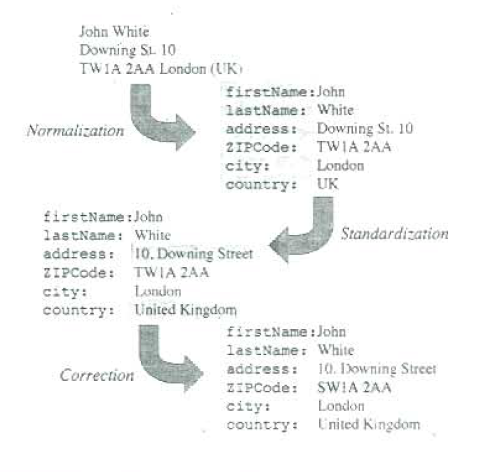
\includegraphics[scale=0.85]{Gambar/transformation}
	\caption{Contoh Proses Transformasi Pada \textit{Data Warehouses}\cite{Matteo:2009}}
	\end{figure} 
Gambar \textbf{2.7} merupakan contoh dari proses \textit{cleansing} dan transformasi dari data pelanggan dimana data berbasis kolom yang terstruktur diekstrak dari sebuah teks yang tidak terstruktur, dengan beberapa nilai kolom distandarisasi sehingga menghilangkan singkatan, dan bahkan nilai dan kolom tersebut saling berkaitan sehingga memudahkan untuk diperbaiki\cite{Matteo:2009}.

\subsubsection{\textit{Loading}}
\textit{Loading} adalah tahap terakhir dari proses ETCL. Kegiatan ini dapat dilakukan dengan dua cara\cite{Matteo:2009}:
\begin{enumerate}
	\item \textit{Refresh}\\
	Data dalam \textit{data warehouse} seluruhnya ditulis ulang, hal ini menandakan data awal diganti dengan data baru. Proses \textit{refresh} biasanya dikombinasikan dengan \textit{static extraction} ketika pertama membangun \textit{data warehouse}.
	\item \textit{Update}\\
	Data yang dimasukan ke dalam \textit{data warehouse} hanya data pada sumber data yang mengalami perubahan atau penambahan saja. \textit{Update} biasanya dilakukan tanpa menghapus atau mengubah data yang ada. Proses \textit{update} biasanya dikombinasikan dengan \textit{incremental extraction} untuk melakukan pembaharuan data secara berkala.
\end{enumerate}

\subsection{Struktur \textit{Data Warehouse } Berdasarkan Konsep Data Multidimensi}

\textit{Data warehouse} merupakan sumber data utama yang akan dianalisis dan diolah menggunakan teknik OLAP. OLAP(\textit{online analytical processing}) menggunakan konsep data multidimensi(terdiri dari banyak dimensi) sehingga struktur \textit{data warehouse} menyerupai kubus (\textit{cube}). Struktur \textit{cube} terdiri dari tiga komponen utama, yaitu \textit{fact, dimension, }dan \textit{measure}. Berikut ini penjelesan mengenai komponen \textit{cube} disertai contoh gambar.\cite{Matteo:2009}

\begin{enumerate}
	\item \textit{Fact}\\
	\textit{Fact} merupakan kumpulan peristiwa (\textit{event}) dalam suatu perusahaan. Contohnya adalah \textit{fact sales} untuk kegiatan penjualan dan \textit{fact shipment} untuk kegiatan pengiriman.
	\item \textit{Dimension} merupakan bagian dari \textit{fact}, namun \textit{dimension} mempunyai lingkup lebih spesifik dari \textit{fact}. Contoh: untuk \textit{fact sales}, terdapat dimensi waktu, produk serta jenis barang.
	\item \textit{Measure}, Merupakan bagian dari \textit{fact}, dimana \textit{measure} biasanya mendeskripsikan \textit{fact} dengan angka atau numerik. Contohnya: \textit{quantity} (banyaknya barang), \textit{unitPrice} (harga per unit), \textit{numberOfCustomer} (banyaknya pelanggan).
\end{enumerate} 

\begin{figure}[h]
	\centering
	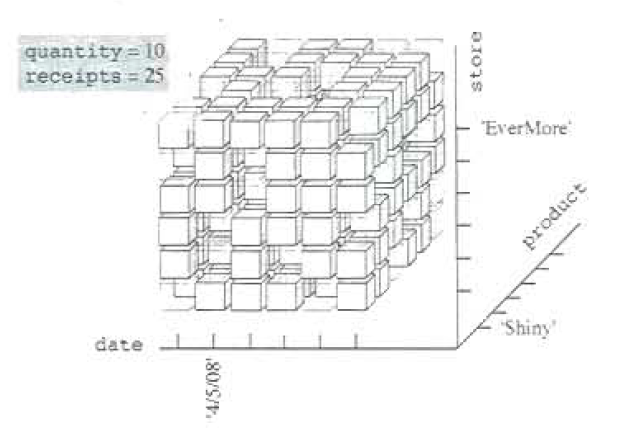
\includegraphics[scale=0.85]{Gambar/contoh-cube}
	\caption{Contoh \textit{Three Dimensional Cube}\cite{Matteo:2009}}
	\end{figure} 

Gambar \textbf{2.8} menggambarkan sebuat \textit{fact sales} memiliki tiga \textit{dimension}, yaitu \textit{date, store, }dan \textit{product}. Serta memiliki dua measure, yaitu \textit{quantity} dan \textit{receipt}. \textit{Cube} tersebut menginformasikan bahwa di toko \textit{EverMore} telah terjual 10 product \textit{Shing} dengan total harga 25 dollar pada tanggal 4 Mei 2008.\cite{Matteo:2009} \\
OLAP mempunyai teknik lain untuk mengolah \textit{cube}, seperti \textit{roll-up, drill-down} dan \textit{slice-dice}.

\begin{figure}[h]
	\centering
	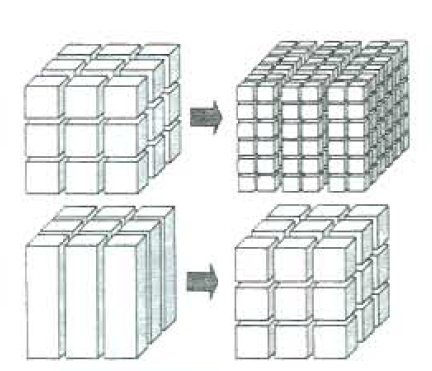
\includegraphics[scale=0.85]{Gambar/drill-down}
	\caption{\textit{Drill-Down}\cite{Matteo:2009}}
	\end{figure} 

Gambar \textbf{2.9} menggambarkan proses \textit{drill-down}. \textit{Drill-down} sendiri merupakan kebalikan dari \textit{roll-up}. Pada gambar \textbf{2.9} teknik \textit{drill-down} digunakan untuk mengurangi agregasi data dan melihat suatu informasi secara lebih detil.

\begin{figure}[h]
	\centering
	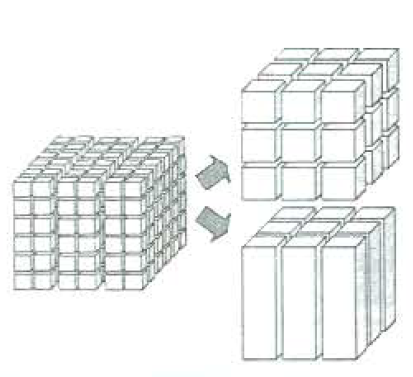
\includegraphics[scale=0.85]{Gambar/roll-up}
	\caption{\textit{Roll-Up}\cite{Matteo:2009}}
	\end{figure} 
	
Gambar \textbf{2.10} menunjukan bahwa \textit{roll-up} digunakan untuk melihat informasi secara umum(\textit{general}).

\begin{figure}[h]
	\centering
	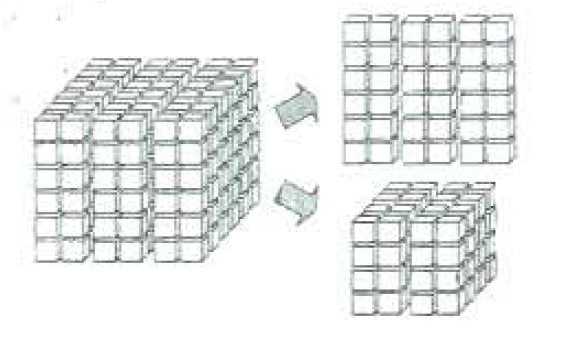
\includegraphics[scale=0.85]{Gambar/slice-dice}
	\caption{\textit{Slice}(Atas) dan \textit{Dice}(Bawah)\cite{Matteo:2009}}
	\end{figure} 

Sedangkan untuk \textit{slice-dice} dapat dilihat pada gambar \textbf{2.11} bahwa \textit{slice} merupakan proses mengurangi \textit{dimension} pada \textit{cube} setelah menempatkan salah satu \textit{dimension} lain menjadi lebih spesifik. \textit{Dice} merupakan proses mengurangi sejumlah data untuk dianalisis dengan cara menyeleksi kriteria tertentu.

\subsection{Teknik Pemodelan Dimensional}
Teknik pemodelan dimensional digunakan untuk menampilkan data dalam \textit{data warehouse}, memungkinkan pengaksesan basis data dengan performansi lebih tinggi, dan membuat struktur basis data menjadi konsisten. \textit{Fact table} berisi beberapa \textit{foreign key} yang berasal dari \textit{dimension} table dan atribut yang berasal dari hasil kalkulasi basis data operasional. \textit{Fact table} berisikan data-data historis, sedangkan \textit{dimension table} memiliki informasi yang mendukung \textit{fact table} dengan format yang lebih spesifik namun masih memiliki \textit{primary key} yang sesuai dengan \textit{fact table}. Pemodelan ini umumnya dijadikan sebagai pendekatan untuk menggambarkan situasi bisnis. Secara umum, terdapat tiga cara pemodelan dimensional, yaitu \textit{star schema, snowflake schema, }dan \textit{constellation schema} \cite{Matteo:2009}.
	\begin{figure}[h]
	\centering
	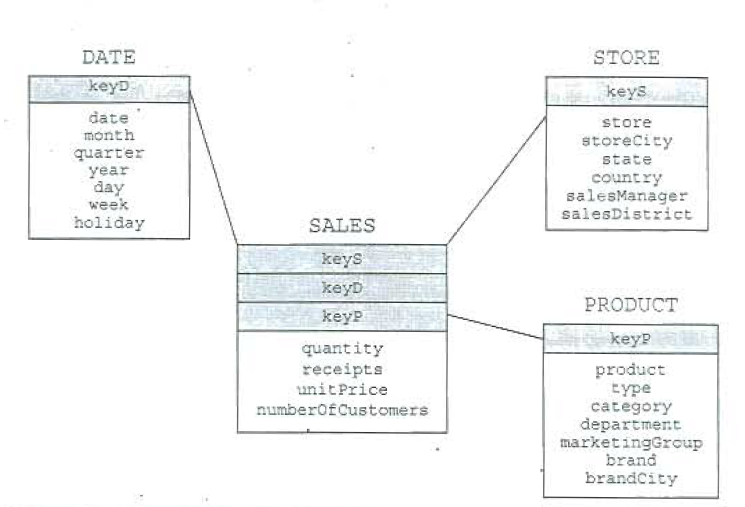
\includegraphics[scale=0.65]{Gambar/star-schema}
	\caption{\textit{Star Schema}\cite{Matteo:2009}}
	\end{figure} 
\begin{enumerate}
	\item \textit{Star schema}\\
	Skema ini terdiri dari sebuah \textit{fact table} yang berhubungan langsung dengan beberapa \textit{dimension table}. Biasanya letak \textit{fact table} berada di tengah dan dikelilingi \textit{dimension} table yang menyerupai bentuk bintang. Keuntungan dari \textit{star schema} ini adalah lebih sederhana sehingga mudah dipahami oleh pengguna. Selain itu, navigasi melalui basis data yang memakai \textit{star schema} lebih optimal dan lebih mudah, meskipun hasil \textit{query} terlihat kompleks.\cite{Matteo:2009}
\item \textit{Snowflake Schema}\\
skema ini adalah variasi bentuk dari \textit{star schema}. Letak perbedaannya ada pada \textit{dimension table}. \textit{Dimension table} pada \textit{star schema} dinormalisasi (memperbaiki desain tabel sehingga penyimpanan data jauh lebih efisien dan bebas anomali data) sehingga menghasilkan tabel baru, namun tetap berhubungan dengan \textit{dimension table} yang bersangkutan. Keuntungan dari skema ini adalah menghemat memori, mengurangi terjadinya redundansi, dan strukturnya yang normal memudahkan proses \textit{update}. Kelemahannya ada pada skema yang dihasilkan kompleks sehingga sulit melakukan pencarian terhadap isi skema. Berikut contoh dari skema \textit{snowflakes}.
  \textit{star schema}.\cite{Matteo:2009}
	\begin{figure}[h]
	\centering
	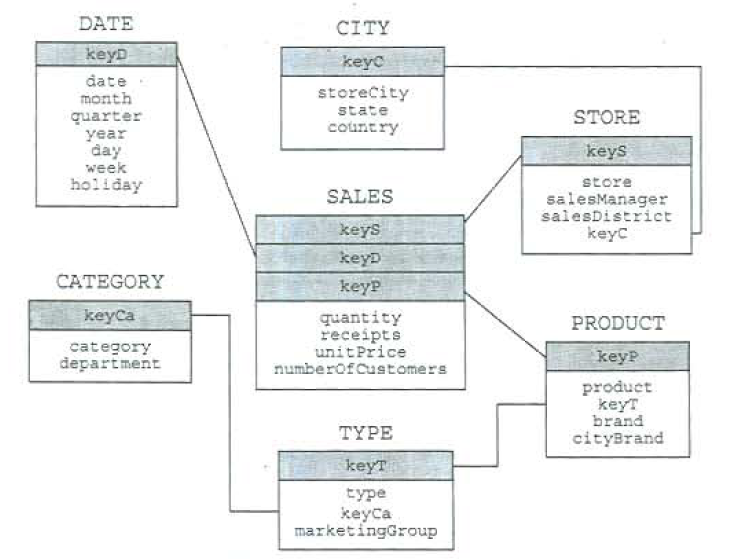
\includegraphics[scale=0.65]{Gambar/snowflakes-schema}
	\caption{\textit{Snowflakes Schema}\cite{Matteo:2009}}
	\end{figure}
	
	\begin{figure}[h]
	\centering
	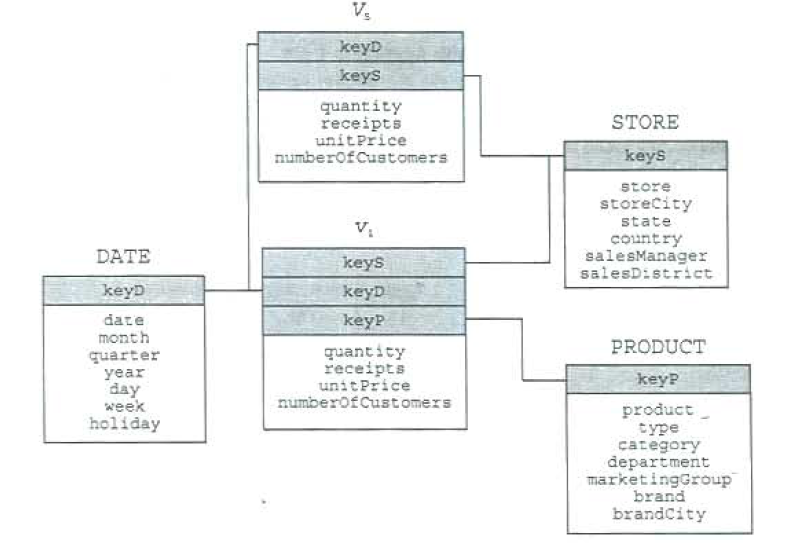
\includegraphics[scale=0.65]{Gambar/constellation-schema}
	\caption{\textit{Constellation Schema}\cite{Matteo:2009}}
	\end{figure}
	
	\item \textit{Constellation schema}\\
	\textit{Constellation schema} merupakan gabungan beberapa \textit{star schema}\cite{Matteo:2009}. Model ini terdiri dari beberapa \textit{fact table} dan saling terbubung dengan \textit{dimension table} bersangkutan. Jadi, sebuah \textit{dimension table} dapat berhubungan dengan dua skema bahkan lebih sehingga menghemat memori dan lebih efektif. Namun, model ini tidak cocok untuk jumlah data yang sangat besar dan kompleks karena memungkinkan proses kalkulasu dari aggregasi data akan memakan waktu yang relatif lama. Berikut contoh skema \textit{Constellation}.
\end{enumerate}

\subsection{Hubungan OLAP, \textit{Data warehouse}, DSS, dengan \textit{Business Intelligence}}
\textit{Data warehouse} akan di olah dengan teknik OLAP agar dapat di analisis dan dievaluasi secara cepat dan efisien. Teknologi OLAP tersebut disediakan oleh BI. Hasil pengolahan \textit{data warehouse} akan dimanfaatkan dalam DSS untuk mengambil keputusan-keputusan penting terkait kepentingan perusahaan. \cite{Matteo:2009}

\section{\textit{Model View Controller}(MVC)}
Setiap perangkat lunak memiliki pola bawaan dalam proses pembuatannya. Salah satu pola yang cukup terkenal adalah konsep MVC. MVC memisahkan pengembangan aplikasi berdasarkan komponen utama yang membangun sebuah aplikasi seperti manipulasi data, user interface, dan bagian yang menjadi kontrol aplikasi. 
\begin{figure}[h]
	\centering
	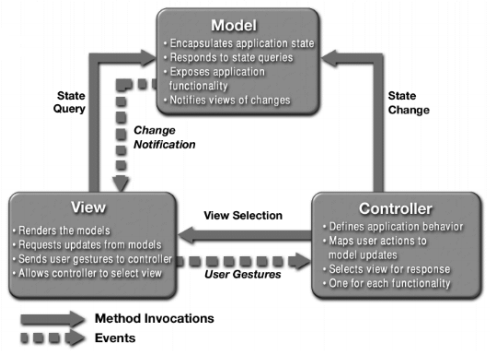
\includegraphics[scale=0.65]{Gambar/MVC}
	\caption{Diagram MVC}
	\end{figure}

Penjelasan MVC sebagai berikut \cite{Hans:2014}:

\begin{itemize}
	\item \textit{Model}\\
	Komponen ini berhubungan dengan proses bisnis yang ada dan juga terdapat di dalam sistem.\\
	Contoh model di ODOO adalah tabel-tabel yang berada di postgresql.
	\item \textit{Controller}\\
	Komponen yang mengatur komponen dari model ke view maupun sebaliknya. Fungsi dari komponen ini adalah sebagai penghubung komponen model dan view.\\
	Contoh \textit{Controller} di ODOO adalah kelas-kelas yang di inisiasi menjadi objek. Setiap kelas yang dibuat harus meng-\textit{extend} kelas osv yang merupakan syarat dari \textit{framework} tersebut.
	\item \textit{View}\\
	komponen yang berhubungan dengan \textit{end user}. Bentuknya berupa tampilan yang akan digunakan oleh \textit{user} atau sering disebut sebagai \textit{user-interface}.
	Contoh \textit{view} di ODOO adalah kode-kode yang dituliskan dalam \textit{file} yang berekstensi xml.\\
	Banyak keuntungan dengan pendekatan MVC, yakni \cite{Hans:2014}:
	\begin{enumerate}
		\item Pembagian modul pengerjaan yang jelas untuk setiap orang di dalam suatu tim.
		\item Kemudahan untuk \textit{maintenance} dimasa depan.
		\item Mempunyai fleksibilitas tinggi dalam pengembangan,
	\end{enumerate}
\footnote{http://elmolya.blogspot.co.id/2010/03/belajar-mvc.html}
	
	
	
\end{itemize}
\section{\textit{Object Relational Mapping}(ORM)}
	
ORM merupakan teknik \textit{programming} yang memetakan basis data relasional ke model objek.Model object dituliskan dalam bentuk bahasa \textit{object-oriented programming} seperti java, C atau python. Pada dasarnya sertiap database yang tersimpan dalam bentuk byte atau array. ORM merubah data di antara berbagai tipe sistem berbeda kedalam database relasional dan OOP. \cite{Hans:2014} \newline 
	Dalam bahasa pemograman yang menggunakan ORM data-data yang tersimpan dalam database aplikasi seperti MySQL atau PostgreSQL, dipetakan menjadi objek sebagai penghubung antara objek yang dibangun dalam program dengan database\footnote{http://www.techopedia.com/definition/24200/object-relational-mapping--orm}, Seperti terlihat pada gambar \textbf{2.16}
	\begin{figure}[h]
	\centering
	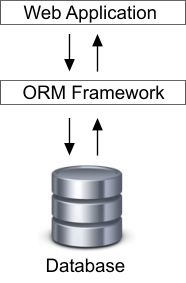
\includegraphics[scale=1]{Gambar/ormFramework}
	\caption{Konsep ORM }
	\end{figure}
	Beberapa keuntungan menggunakan ORM, diantaranya: \footnote{http://www.techopedia.com/definition/24200/object-relational-mapping--orm}
	\begin{enumerate}
		\item Pengembangan menjadi lebih sederhana karena ORM mengotomatisasi konversi objek kedalam tabel maupun sebaliknya. Hasil dalam pengembangan ini adalah biaya pemeliharaan yang lebih rendah.
		\item Mengurangi penulisan code untuk pemanggilan SQL dan prosedur penyimpanan data dalam database.
		\item Meningkatkan performansi sistem.
		\item Solusi optimal yang dapat membuat sistem menjadi lebih cepat dan mudah dalam pemeliharaan sistem.
	\end{enumerate}
	
	
	\section{Framework ODOO} 
	
	ODOO adalah aplikasi open source guna memanajemen ERP sebuah usaha atau lebih tepatnya ERP sebuah perusahaan. ODOO memiliki tampilan yang cukup minimalis. Didalamnya tercantum manajemen penjualan, logistik, akutansi, pemberdayaan pekerja, dan produksi. Dengan sebuah aplikasi ODOO diharap ERP sebuah perusahaan dapat dijalankan semaksimum mungkin tanpa mengurangi unsur-unsur lain dalam usaha didalamnya.\footnote{https://doc.odoo.com/}

\subsection{Arsitektur ODOO}

Bagian ini menyajikan arsitektur ODOO bersama dengan rincian teknologi aplikasi. Disajikan tingkatan penyusunan ODOO, sarana komunikasi dan protokol antara komponen aplikasi. Seperti terlihat pada gambar \textbf{2.17}

\subsubsection{\textit{Client-Server Architecture}}
ODOO memiliki komponen \textit{client server} terpisah, dengan kata lain
Server berjalan secara terpisah dari klien. Server menangani logika bisnis dan berkomunikasi dengan aplikasi database, sedangkan
klien menyajikan informasi kepada pengguna dan memungkinkan pengguna untuk beroperasi dengan aplikasi server.Disisi lain ODOO menyediakan multiple klien.

	\begin{figure}[H]
	\centering
	\includegraphics[scale=0.4]{Gambar/arsitekturODOO2}
	\caption{Arsitektur ODOO }
	\end{figure}


\subsubsection{Server dan Modul}
Server ODOO ditulis dalam bahasa pemrograman Python. Klien berkomunikasi dengan server dengan menggunakan antarmuka XML-RPC, sedangkan fungsi bisnis  diatur dalam modul. Modul adalah folder dengan yang telah ditentukan struktur yang berisi kode dan XML \textit{Python file}. Sebuah modul mendefinisikan struktur data, \textit{form}, laporan, menu, prosedur, dan alur kerja. Modul didefinisikan menggunakan sintaks \textit{client-independent}. Jadi, menambahkan objek baru, seperti menu atau bentuk, serta membuatnya tersedia untuk klien.\footnote{https://doc.odoo.com/}

\subsubsection{Aplikasi Klien}
Dua aplikasi Client adalah:\footnote{https://doc.odoo.com/}
\begin{enumerate}
	\item Sebuah Aplikasi web yang digunakan sebagai HTTPserver memungkinkan pengguna untuk terhubung menggunakan web browser.  
	\item Desktop aplikasi yang ditulis dalam Python yang menggunakan GTK (\textit{Graphics tool Kit})
\end{enumerate}

\subsubsection{Database} 
ODOO menggunakan PostgreSQL sebagai sistem manajemen database. PostgreSQL adalah sistem manajemen database objek-relasional (ORDBMS)\\ 
\textit{Report}:\footnote{https://doc.odoo.com/} \\
ODOO juga menyediakan sistem pelaporan dengan integrasi OpenOffice.org memungkinkan kustomisasi laporan. 
OpenOffice.org dengan komponen utamanya adalah untuk pengolah kata, \textit{spreadsheet}, presentasi, grafis, dan \textit{database}.

\subsubsection{Tiga Tingkatan Arsitektur DOO}
ODOO adalah \textit{multitenant} dengan tiga tingkatan arsitektur : \textit{Database tier} untuk penyimpanan data, \textit{application tier} untuk pengolahan dan \textit{functionalities}dan \textit{presentation tier} menyediakan antarmuka pengguna. \textit{Database, application, functionalities,} dan \textit{presentation} adalah lapisan yang terpisah dalam ODOO. \textit{Application tier} sendiri ditulis sebagai inti; beberapa modul tambahan dapat diinstal dalam rangka menciptakan spesifikasi khusus dari ODOO yang disesuaikan dengan kebutuhan dan persyaratan khusus. Selain itu, ODOO mengadopsi pola arsitektur Model-View-Controller (MVC).\footnote{https://doc.odoo.com/}

Untuk mengakses ODOO dapat dilakukan dengan cara:\footnote{https://doc.odoo.com/}
\begin{enumerate}
	\item menggunakan browser web menunjuk klien-server web ODOO, atau
	\item menggunakan aplikasi client (klien GTK) diinstal pada setiap komputer.
\end{enumerate}
Dua metode akses memberikan fasilitas yang sangat mirip, dan dapat menggunakan kedua akses server yang sama pada waktu yang sama. Cara terbaik adalah dengan menggunakan web browser jika server ODOO adalah agak jauh (seperti di benua lain) karena lebih toleran terhadap penundaan waktu antara dua dari klien GTK adalah. Klien web juga lebih mudah untuk mempertahankan, karena umumnya sudah diinstal pada komputer pengguna.\footnote{https://doc.odoo.com/}
Sebaliknya akan lebih baik dengan klien aplikasi (disebut klien GTK karena teknologi itu dibangun dengan) menggunakan server lokal (seperti di gedung yang sama). Dalam hal ini klien GTK akan lebih responsif, sehingga lebih memuaskan untuk digunakan.\footnote{https://doc.odoo.com/} \\

Ada sedikit perbedaan fungsional antara dua klien ODOO - klien web dan klien GTK saat ini. Klien web menawarkan fungsionalitas yang lebih, misalnya, fitur Intelijen Perusahaan, dan tampilan Gantt.
Ketika  mengubah struktur instalasi ODOO (menambah dan menghapus modul, mungkin mengubah label), mungkin menemukan klien web menjadi tidak tepat karena penggunaannya \textit{caching}.\footnote{https://doc.odoo.com/}\\
\textit{Caching} mempercepat semuanya dengan menjaga salinan data di suatu tempat antara server dan klien, yang biasanya baik. Tapi mungkin telah membuat perubahan pada instalasi bahwa   tidak dapat langsung melihat di browser. Banyak kesalahan yang jelas disebabkan oleh perubahan struktur instalasi ODOO, Solusinya adalah dengan menggunakan klien GTK selama pengembangan dan implementasi di mungkinkan. \\
Perusahaan ODOO akan terus mendukung dua klien, yaitu \textit{web browser}, GTK di masa mendatang, sehingga dapat menggunakan klien yang di inginkan.\footnote{https://doc.odoo.com/} \\
Sebuah penyebaran khas ODOO ditampilkan pada Gambar \textbf{2.18} . Penyebaran ini disebut Web tertanam penyebaran. Seperti ditunjukkan, sistem ODOO terdiri dari tiga komponen utama:
\begin{enumerate}
	\item server PostgreSQL database, yang berisi semua database, yang masing-masing berisi semua data dan sebagian besar elemen konfigurasi sistem ODOO.
	\item server aplikasi ODOO, yang berisi semua logika perusahaan dan memastikan bahwa ODOO berjalan secara optimal.
	\item server web, aplikasi terpisah yang disebut Open Object client-web, yang memungkinkan   untuk terhubung ke ODOO dari browser web standar dan tidak diperlukan saat menghubungkan menggunakan klien GTK.
\end{enumerate}
	\begin{figure}[H]
	\centering
	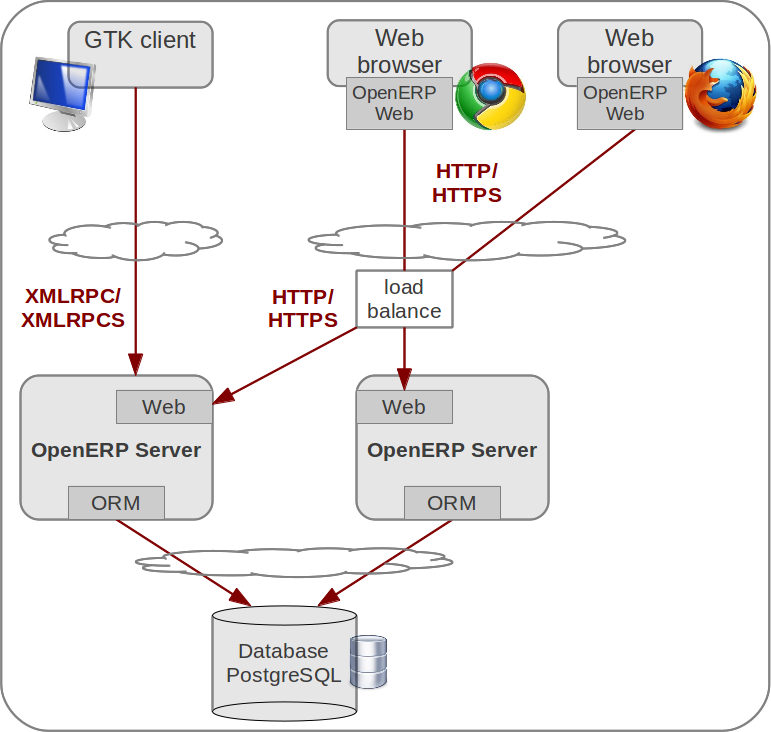
\includegraphics[scale=0.4]{Gambar/arsitekturOdoo3}
	\caption{Arsitektur ODOO}
	\end{figure}

\subsubsection{\textit{Database} PostgreSQL}
\textit{Tier}data ODOO disediakan oleh database relasional PostgreSQL. Sementara query SQL langsung dapat dijalankan dari modul ODOO, sebagian mengakses ke database relasional dilakukan melalui server Object lapisan Pemetaan Relasional.
Database berisi semua data aplikasi, dan juga sebagian besar elemen konfigurasi sistem  ODOO. Perhatikan bahwa server ini mungkin dapat digunakan menggunakan database berkerumun.\footnote{https://doc.odoo.com/}

\subsubsection{Server ODOO }
 ODOO menyediakan server aplikasi yang aplikasi bisnis tertentu dapat dibangun. Ini juga merupakan kerangka pengembangan yang lengkap, menawarkan berbagai fitur untuk menulis aplikasi mereka. Di antara fitur tersebut,  ODOO ORM menyediakan fungsionalitas dan antarmuka di atas server PostgreSQL. Server  ODOO juga dilengkapi dengan lapisan khusus yang dirancang untuk berkomunikasi dengan klien berbasis browser web. Lapisan ini menghubungkan pengguna dengan menggunakan \textit{browser standard} untuk server.
Dari perspektif pengembang, server bertindak baik sebagai perpustakaan yang membawa manfaat di atas sementara menyembunyikan rincian tingkat rendah, dan sebagai cara sederhana untuk menginstal, mengkonfigurasi dan menjalankan aplikasi yang ditulis. Server juga berisi layanan lainnya, seperti \textit{model extensible}data dan tampilan, mesin alur kerja atau mesin laporan. Namun, mereka adalah layanan  ODOO tidak secara khusus terkait dengan keamanan, dan karena itu tidak dibahas secara rinci dalam dokumen ini.\footnote{https://doc.odoo.com/}

\subsubsection{Server - ORM}

Objek Relational Mapping ORM lapisan adalah salah satu fitur yang menonjol dari  ODOO Server. Ini menyediakan fungsionalitas tambahan dan penting di atas server PostgreSQL. Model Data dijelaskan dalam Python dan  ODOO menciptakan tabel database yang mendasari menggunakan ORM ini. Semua manfaat RDBMS seperti kendala yang unik, integritas relasional atau query efisien digunakan dan dilengkapi dengan fleksibilitas Python. Misalnya, kendala yang sewenang-wenang ditulis dengan Python dapat ditambahkan ke model apapun. Mekanisme diperpanjang modular berbeda juga diberikan oleh  ODOO.\footnote{https://doc.odoo.com/}\\
Hal ini penting untuk memahami tanggung jawab ORM sebelum mencoba untuk by-pass dan untuk mengakses langsung database yang mendasari melalui query SQL baku. Bila menggunakan ORM,  ODOO dapat memastikan data tetap bebas dari korupsi apapun. Misalnya, sebuah modul dapat bereaksi terhadap penciptaan data dalam tabel tertentu. Perilaku ini dapat terjadi hanya jika pertanyaan melalui ORM.
Layanan yang diberikan oleh ORM antara lain:\footnote{https://doc.odoo.com/}
\begin{enumerate}
	\item konsistensi validasi oleh pemeriksaan validitas kuat.
	\item menyediakan sebuah antarmuka pada objek (metode, referensi, ...) yang memungkinkan untuk merancang dan mengimplementasikan modul efisien.
	\item keamanan tingkat baris per pengguna dan kelompok; Rincian lebih lanjut tentang pengguna dan kelompok pengguna diberikan dalam Pengguna bagian dan Peran Pengguna.
	\item tindakan yang kompleks pada sekelompok sumber daya.
	\item Layanan warisan memungkinkan pemodelan baik sumber daya baru.
\end{enumerate}

\subsubsection{Server - Web}
Lapisan web menawarkan antarmuka untuk berkomunikasi dengan browser standar. Dalam versi 6.1 dari  ODOO, web-client telah ditulis ulang dan diintegrasikan ke dalam server tier  ODOO. Lapisan web ini adalah aplikasi WSGI kompatibel berdasarkan Schieberegler. Ini menangani permintaan http biasa ke file server statis atau konten dinamis dan permintaan JSON-RPC untuk RPC terbuat dari browser.\footnote{https://doc.odoo.com/}

\subsubsection{Modul}

Server ODOO merupakan \textit{core} didalam arsitektur ODOO. Untuk setiap perusahaan, nilai  ODOO terletak pada modul yang berbeda. Peran modul adalah untuk mengimplementasikan kebutuhan bisnis. Server adalah satu-satunya komponen yang diperlukan untuk menambahkan modul.Setiap rilis  ODOO resmi mencakup banyak modul, dan ratusan modul yang tersedia. Contoh modul tersebut Akun, CRM, HR, Pemasaran, MRP, Sale, dll
Klien.\footnote{https://doc.odoo.com/}
Modul berperan sebagai \textit{application logic} yang terkandung dalam \textit{server-side} serta klien secara konseptual yang sederhana. Modul mengeluarkan permintaan ke server, mendapatkan data kembali dan menampilkan hasilnya (misalnya daftar pelanggan) dengan cara yang berbeda (seperti bentuk, daftar, kalender, ...). Setelah ada tindakan dari pengguna, modul akan mengirimkan permintaan untuk memodifikasi data ke server.
Klien default  ODOO adalah aplikasi JavaScript yang berjalan di browser yang berkomunikasi dengan server dengan menggunakan JSON-RPC.\footnote{https://doc.odoo.com/}

\subsubsection{Arsitektur MVC di ODOO}
\textit{Model-view-controller}(MVC) adalah pola arsitektur yang digunakan dalam rekayasa perangkat lunak". Dalam aplikasi komputer yang kompleks menyajikan banyak data kepada pengguna, kita sering ingin memisahkan data (model) dan \textit{user interface}(\textit{view}). Perubahan \textit{user interface} tidak berdampak terhadap manajemen data, dan data dapat ditata kembali tanpa mengubah antarmuka pengguna. \textit{Model-view-controller}memecahkan masalah tersebut dengan \textit{decoupling} akses data dan logika bisnis dari penyajian data dan interaksi pengguna, dengan memperkenalkan komponen menengah yang disebut \textit{controller}.\footnote{https://doc.odoo.com/}
 
\begin{figure}[h]
	\centering
	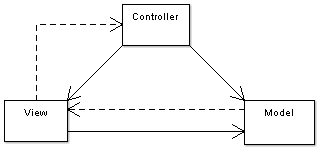
\includegraphics[scale=1]{Gambar/DiagramMVC}
	\caption{Diagram MVC}
	\end{figure}

Pada tampilan diagram di atas, garis tebal untuk panah mulai dari \textit{controller}, \textit{view} dan \textit{Model}, itu berarti bahwa \textit{controller} memiliki akses lengkap terhadap \textit{view} dan \textit{Model}. Garis putus-putus untuk panah sebalikbta dari \textit{view} ke controller berarti bahwa \textit{view} memiliki akses terbatas terhadap controller.\\
Alasan dari desain ini adalah:\footnote{https://doc.odoo.com/}
\begin{enumerate}
	\item Dari View ke Model: \textit{Model} mengirimkan pemberitahuan terhadap \textit{view} ketika data yang telah dimodifikasi. \textit{Model} ini tidak memerlukan \textit{inner view} untuk melakukan operasi ini. Namun, \textit{view} perlu mengakses bagian internal dari \textit{Model}.
	\item Dari View Controller: alasan mengapa \textit{view} memiliki akses terbatas ke controller adalah karena ketergantungan dari \textit{view} ke controller seminimal mungkin sehingga controller dapat diganti setiap saat.
\end{enumerate}

ODOO mengikuti MVC semantik dengan
\begin{enumerate}
	\item \textit{Model}: Tabel PostgreSQL.
	\item \textit{view}: \textit{view} yang didefinisikan dalam file XML di ODOO.
	\item \textit{Controler}: Objek ODOO.
\end{enumerate}

